\documentclass[11pt]{article}
\usepackage{mathtools}
\usepackage{mdframed}
\usepackage{fullpage}
\usepackage{amsfonts}
\usepackage{tikz}
\usepackage{fancyhdr}
\usepackage{lastpage}
\usepackage{graphicx}

\graphicspath{{coms574/hw2/}}

%edit this for each class
\newcommand\name{John Collin Vincent}
\newcommand\classname{Com S 474}
\newcommand\assignment{Homework 2}


\newcounter{excounter}
\setcounter{excounter}{1}
\newcommand\ques[2]{\vskip 1em  \noindent\textbf{\arabic{excounter}\addtocounter{excounter}{1}.} \emph{#1} \noindent#2}
\newenvironment{question}{\ques{}\begin{quote}}{\end{quote}}
\newenvironment{subquestion}[1]{#1) \begin{quote}}{\end{quote}}

\pagestyle{fancy}
\rfoot{\name, page \thepage/\pageref{LastPage}}
\cfoot{}
\rhead{}
\lhead{}
\renewcommand{\headrulewidth}{0pt}
\renewcommand{\footrulewidth}{0pt}
\DeclarePairedDelimiter\ceil{\lceil}{\rceil}
\DeclarePairedDelimiter\floor{\lfloor}{\rfloor}


\begin{document}


    {\bf \classname \hspace{1cm} \assignment\hfill \name}
    \vskip 2em


    \begin{question}
        \begin{align*}
            Y_i &= m(x_i)+e_i \\
            e_i &= Y_i - m(x_i) \\
            e^{2}_{i} &= (Y_i - m(x_i))^2 \\
            \sum_{i=1}^{n} e^2_i &= \sum_{i=1}^{n} (Y_i - m(x_i))^2 \\
            RSS = \sum_{i=1}^{n} e^2_i &= \sum_{i=1}^{n} (Y_i - m(x_i))^2 & 
                \text{by definition in textbook page 62}\\
            RSE &= \hat{\sigma_e}\\
            RSE &= \sqrt{\frac{RSS}{(n-2)}} & \text{book page 66}\\
            \hat{\sigma}^2_e &= \frac{RSS}{(n-2)} = \frac{\sum_{i=1}^{n} (Y_i - m(x_i))^2}{(n-2)}\\
        \end{align*}
    \end{question}
    
    \clearpage

    \begin{question}
        \begin{center}\underline{Linear $X$}\end{center}
            \begin{figure}[h]
                \centering
                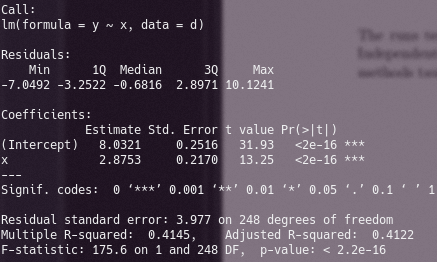
\includegraphics[width=0.8\textwidth]{xsummary.png}\\
                \mbox{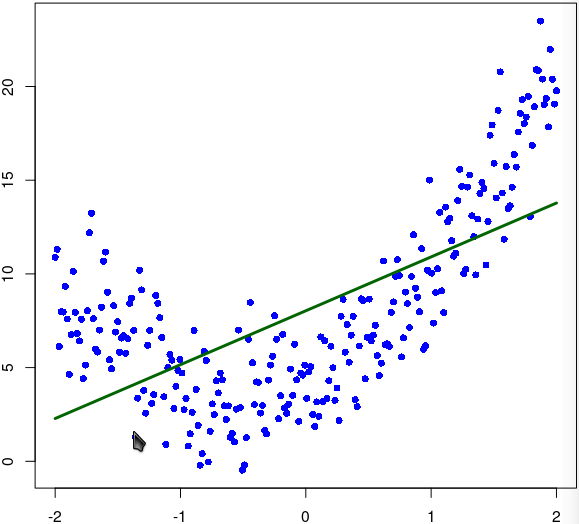
\includegraphics[width=0.45\textwidth]{xgraph.png}}
                \hspace{30px}
                \mbox{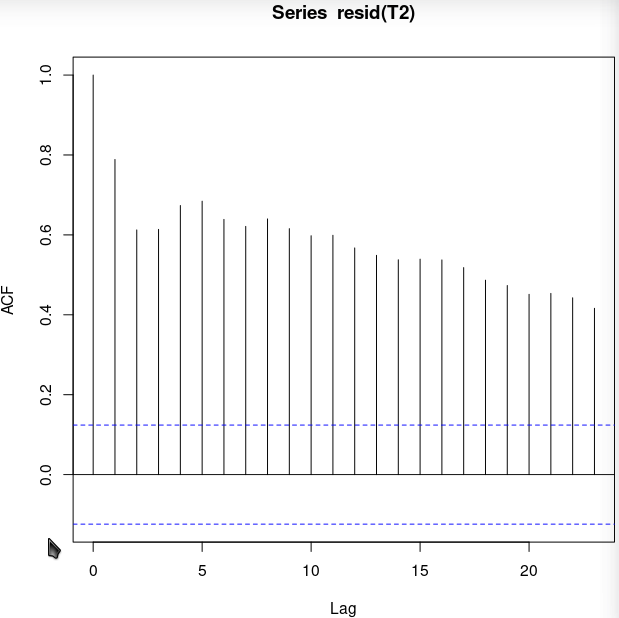
\includegraphics[width=0.45\textwidth]{xafc.png}}
                \caption{R output for $x$}
            \end{figure}
            The runs test results in a p-value less than 2.2e-16  which means that the errors are not
            Independent. This means that we cannot prove this model is the optimal model through
            methods taught in this class.
        \clearpage

        \begin{center}\underline{$X^2$}\end{center}
            \begin{figure}[h]
                \centering
                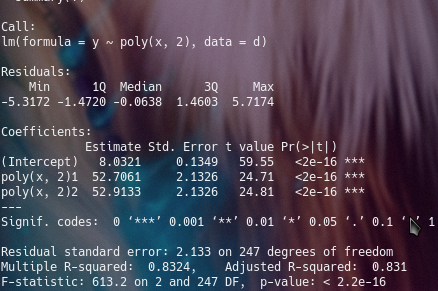
\includegraphics[width=0.8\textwidth]{x2summary.png}\\
                \mbox{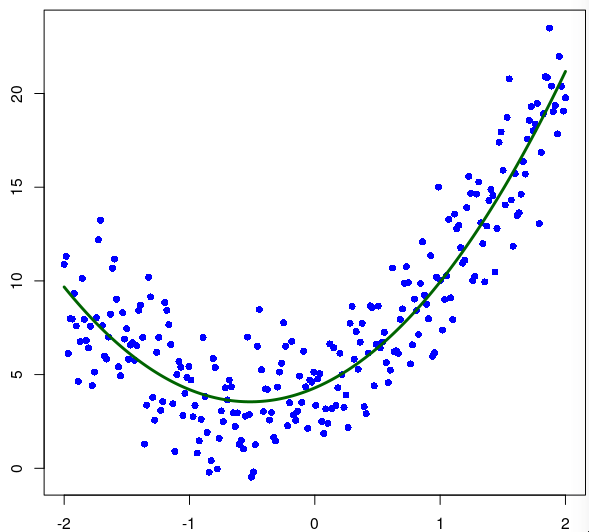
\includegraphics[width=0.45\textwidth]{x2graph.png}}
                \hspace{30px}
                \mbox{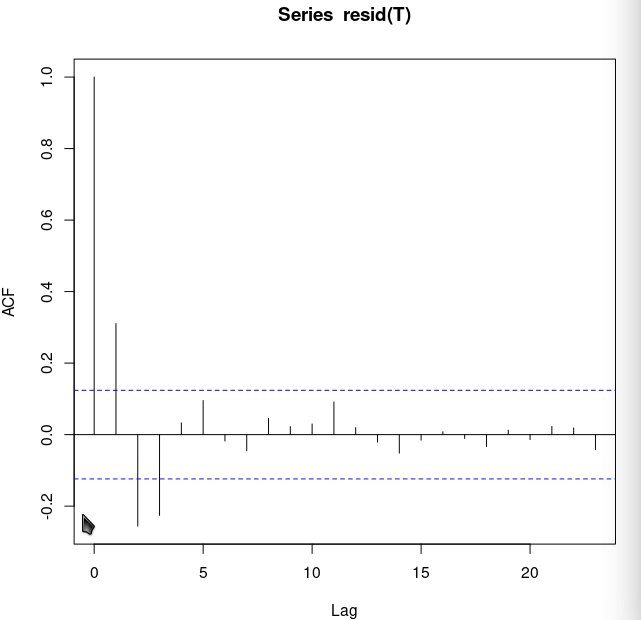
\includegraphics[width=0.45\textwidth]{x2afc.png}}
                \caption{R output for $x^2$}
            \end{figure}
            The runs test results in a p-value of 0.0003869 which means that the errors are not
            Independent. This means that we cannot prove this model is the optimal model through
            methods taught in this class.

        \clearpage

        \begin{center}\underline{$X^3$}\end{center}
        
            \begin{figure}[h]
                \centering
                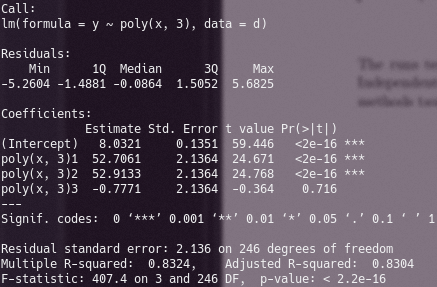
\includegraphics[width=0.75\textwidth]{x3summary.png}\\
                \mbox{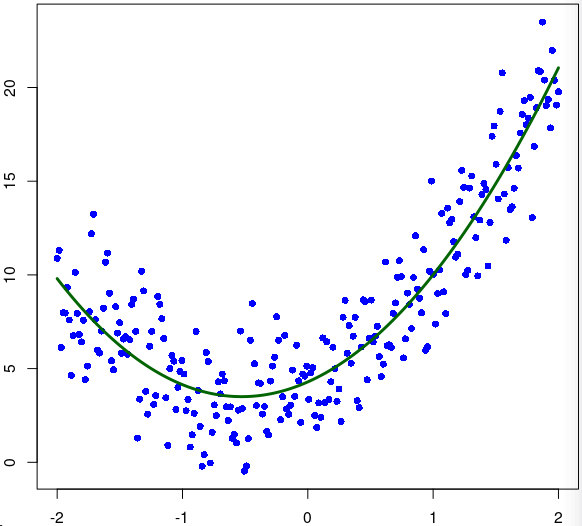
\includegraphics[width=0.4\textwidth]{x3graph.png}}
                \hspace{30px}
                \mbox{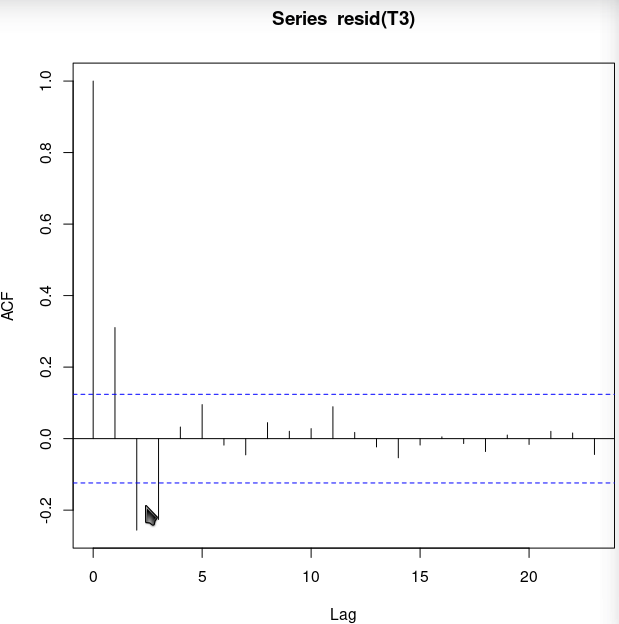
\includegraphics[width=0.4\textwidth]{x3afc.png}}
                \caption{R output for $x^3$}
            \end{figure}
            The runs test results in a p-value of 0.0003869 which means that the errors are not
            Independent. This means that we cannot prove this model is the optimal model through
            methods taught in this class.
        
        \clearpage

        \begin{center}\underline{Summary}\end{center}
        
            Just by looking at the first plot with x being linear you can see that it does not
            match the data very well for almost the entire plot. the residuals are also pretty
            high throughout. The $R^2$ is also pretty low at .41\\
            The $x^2$ plot clearly matches the data much better. It also has min and max residuals 
            that are much closer to 0 and a median that is 10 times lower. It's $R^2$ is double
            that of the previous model proving that it is a much better fit.\\
            The $X^3$ plot is actaully identical to the $X^3$ plot which kind of supprised
            me. Clearly increasing the complexity of the model does not have any benifit.
            Based on these findings I would recommend a $X^2$ model for this data.
    \end{question}

\end{document}
